\subsection{A deblending test}
\label{sec:deblending_test}

TODO: here, I look at results on a small $8 \times 8$ image. 

Preliminary results are in 


\begin{figure}[!htb]
    \centering
    \begin{subfigure}[t]{0.9\textwidth}
    \centering
    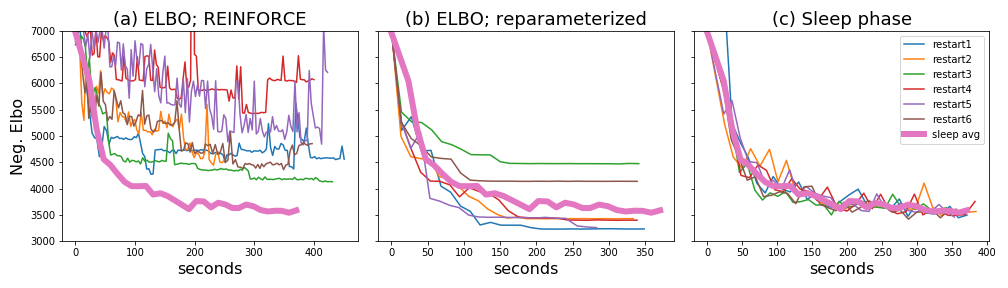
\includegraphics[width=\textwidth]{figures/optim_path_compare.png}
    \end{subfigure}
    \begin{subfigure}[t]{\textwidth}
    \centering
    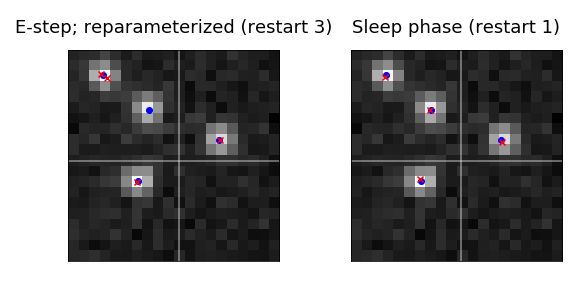
\includegraphics[width=0.55\textwidth]{figures/optim_path_detect_compare.png}
    \end{subfigure}
    \vspace{-3em}
    \caption{(Top) The ELBO as the optimization progresses, for six random restarts. Bold pink line in all plots is the sleep phase ELBO path, averaged over six restarts. (Bottom) MAP locations from two variational posteriors shown in red. On the left, the detections from restart 3 of using the reparameterized gradient, where the optimization got stuck in local optima. All posteriors optimized with the sleep phase posteriors correctly detected four stars. Restart 1 is shown on the right. }
    \label{fig:optim_path}
\end{figure}
